\documentclass[twoside,10pt]{article}
\usepackage{amsmath,amsfonts,amsthm,fullpage}
\usepackage{algorithm}
\usepackage{algorithmic}
\usepackage{graphicx}
\usepackage{float}
\usepackage{multirow}
\usepackage{subcaption}
\usepackage[colorlinks=true, hidelinks]{hyperref}
\usepackage{enumitem}
\usepackage{tcolorbox}
\hypersetup{
    colorlinks=true,
    linkcolor=blue,
    citecolor=blue,
}
\usepackage{listings}
\usepackage{xcolor}

\definecolor{codegreen}{rgb}{0,0.6,0}
\definecolor{codegray}{rgb}{0.5,0.5,0.5}
\definecolor{codepurple}{rgb}{0.58,0,0.82}
\definecolor{backcolour}{rgb}{0.95,0.95,0.92}

% \makeatletter
% \renewcommand{\@makefnmark}{%
%   \hbox{%
%     \@textsuperscript{%
%       \normalfont\color{blue}(\@thefnmark)%
%     }%
%   }%
% }
% \makeatother

\lstdefinestyle{mystyle}{
    backgroundcolor=\color{backcolour},   
    commentstyle=\color{codegreen},
    keywordstyle=\color{magenta},
    numberstyle=\tiny\color{codegray},
    stringstyle=\color{codepurple},
    basicstyle=\ttfamily\footnotesize,
    breakatwhitespace=false,         
    breaklines=true,                 
    captionpos=b,                    
    keepspaces=true,                 
    numbers=left,                    
    numbersep=5pt,                  
    showspaces=false,                
    showstringspaces=false,
    showtabs=false,                  
    tabsize=2
} 

\lstset{style=mystyle}

\usepackage[backend=biber,style=alphabetic,sorting=ynt]{biblatex}
\addbibresource{references.bib}



\begin{document}

\title{ISYE 6740 Fall 2025\\ Homework 2 \\
(100 points + 5 bonus points)}
\author{William Pickard}
\date{}

\maketitle

\textbf{Provided Data:}
Questions marked with GS must be submitted to Gradescope. You must still include all your results and explanations in this PDF, and include your code in your submitted zip. Failure to pass all gradescope tests will result in losing 50\% of the points for that question.

\begin{itemize}
    \item (GS) Q3: Order of faces using ISOMAP [isomap.dat, isomap.mat]
    \item (GS) Q4: Eigenfaces and simple face recognition [yalefaces]
\end{itemize}

\leavevmode\newline
\textbf{All results that are present only in code/notebooks, but not in your PDF report will not be accepted for points.}\\
\textbf{Handwritten solutions will not be accepted for any reason}\\
\textbf{For any code that requires randomness, please set your seed as 6740}

\subsection*{1. Conceptual questions [30 points].}


\begin{enumerate}

\item (5 points) Please prove the first principle component direction $v$ corresponds to the largest eigenvalue of the sample covariance matrix:
\[
v = \arg\max_{w: \|w\|\leq 1} \frac 1 m \sum_{i=1}^m (w^T x^i - w^T \mu)^2.
\]
You may use the proof steps in the lecture, but please write them logically and cohesively.
\subsection*{1.1 PCA Proof}
This objective function tries to find a vector $w$ that maximizes the variance. To begin, we will manipulate the objective function to a form that can be reduced.
\begin{align}
\frac 1 m \sum_{i=1}^m (w^T x^i - w^T \mu)^2 &= \frac 1 m \sum_{i=1}^m (w^T (x^i - \mu))^2 \\
&= \frac 1 m \sum_{i=1}^m w^T(x^i - \mu)w^T(x^i - \mu) \\
\intertext{Using inner product property:}   a^Tb &= b^Ta \\
&= \frac 1 m \sum_{i=1}^m w^T(x^i - \mu)(x^i - \mu)^Tw \\\
\intertext{Factor out w since it is independent of i}: \\
&= w^T(\frac 1 m \sum_{i=1}^m (x^i - \mu)(x^i - \mu)^T)w \\
\intertext{Now, we can substitute the given covariance matrix equation: } \\  C &= \frac 1 m \sum_{i=1}^m (x^i - \mu)(x^i - \mu)^T \\
\frac 1 m \sum_{i=1}^m (w^T x^i - w^T \mu)^2 &= w^TCw \label{eq:reduced_obj}
\end{align}

With this simplified form, we can follow a common strategy for solving constrained optimization problems: the Lagrangian function. 
The constraint on this problem will be that $w$ cannot exceed 1 in magnitude. This must be done, since w is multiplied
by itself in the objective function, and without a constraint, the objective function can be made arbitrarily large without a constraint.

With the Lagrangian function, we will take the derivative and set it to zero.

\begin{align}
L(w, \lambda) &= w^TCw + \lambda (1- ||w||^2) \\
\frac {\partial L} {\partial w} = 0 &= \frac{\partial (w^TCw)}{\partial w} + \frac{\partial \lambda}{\partial w} - \frac{\partial (\lambda ||w||^2)}{\partial w} \\
\intertext{Using the formula for a quadratic form derivative \cite[Eq. 81]{Petersen2008}: $\frac{\partial (x^TBx)}{dx} = (B + B^T)x$} \\
\intertext{ and derivative of the matrix L2 norm \cite[Eq. 131]{Petersen2008}: $\frac {\partial ||x||^2_2}{\partial x} = 2x$} \\
&= (C+C^T)x - 2\lambda w \\
\intertext{Considering that the covariance matrix is symmetrical, so $C = C^T$} \\
0 &= 2Cw -2\lambda w \\
Cw &= \lambda w
\end{align}

At the end of the optimization, we find that it is the same equation as the eigenvalue equation $Av=\lambda v$ with $\lambda$ being the eigenvalue and $w$ being the eigenvector. 
Therefore, the optimal solution $w$ is an eigenvector of $C$. Further, if we input the optimized value $\lambda w$ into the reduced objective function \eqref{eq:reduced_obj}, we find that 
the eigenvector $w$ that maximizes the variance of the projection corresponds to the largest eigenvalue $\lambda$.

\begin{align}
    \frac 1 m \sum_{i=1}^m (w^T x^i - w^T \mu)^2 = w^TCw &= w^T(\lambda w)
    \intertext{From our constraint, we know $w^Tw = 1$}
    v = \arg\max_{w: \|w\|\leq 1} \frac 1 m \sum_{i=1}^m (w^T x^i - w^T \mu)^2 &= \lambda
\end{align}
\item (5 points) Based on your answer to the question above, explain how to further find the second and third largest principle component directions.
\subsection*{1.2 PCA Continued}
If the first principal component corresponds to the largest eigenvalue, the following components correspond to the following eigenvectors in order of their corresponding eigenvalues' magnitude. These directions are orthogonal to each other, and since they're taken in order of the corresponding largest eigenvalues, each additional eigenvector maximizes the remaining variance that has not already been projected.
\item (5 points) 
Consider the diagonal matrix \( A = \begin{bmatrix} 3 & 0 \\ 0 & 2 \end{bmatrix} \).  
Find two distinct eigenvalue decompositions of \( A \), and prove mathematically that both are valid. This demonstrates that eigendecomposition is not unique. \textbf{Note:} Your eigenvalue decompositions must be done mathematically, not programatically.
\subsection*{1.3 Eigendecomposition}
Find the eigenvalues:
\begin{align*}
det (A-\lambda I) = \det \begin{bmatrix} 3-\lambda & 0 \\ 0 & 2-\lambda \end{bmatrix} &= 0 \\
(3-\lambda)(2-\lambda) &= 0 \\
\lambda_1 = 3, \lambda_2 &= 2
\end{align*}
Find the eigenvectors:
\begin{align*}
\intertext{For $\lambda_1$:}
(A-3I)v = \begin{bmatrix} 0 & 0 \\ 0 & -1 \end{bmatrix}v  &= 0 \\
v_1 \text{is free, } v_2 = 0 \\
v_1 = \begin{bmatrix} 1 \\ 0 \end{bmatrix}
\intertext{For $\lambda_2$:}
(A-2I)v = \begin{bmatrix} 1 & 0 \\ 0 & 0 \end{bmatrix}v  &= 0 \\
v_1 = 0 \text{, } v_2 \text{ is free} \\
v_2 = \begin{bmatrix} 0 \\ 1 \end{bmatrix}
\end{align*}
Prove the first decomposition using $A = P^1D^1P^{-1}$. $P^1$ is the matrix of eigenvectors, $D^1$ is the diagonal matrix of eigenvalues. 
\begin{align*}
A= \begin{bmatrix} 3 & 0 \\ 0 & 2 \end{bmatrix}, \quad P^1 = \begin{bmatrix} 1 & 0 \\ 0 & 1 \end{bmatrix}, \quad D^1 &= \begin{bmatrix} 3 & 0 \\ 0&2 \end{bmatrix} \\
\begin{bmatrix} 3 & 0 \\ 0 & 2 \end{bmatrix} &= \begin{bmatrix} 1 & 0 \\ 0 & 1 \end{bmatrix} \begin{bmatrix} 3 & 0 \\ 0&2 \end{bmatrix} \begin{bmatrix} \frac 1 1 & 0 \\ 0 & \frac 1 1 \end{bmatrix} \\
\begin{bmatrix} 3 & 0 \\ 0 & 2 \end{bmatrix} &= \begin{bmatrix} 3 & 0 \\ 0&2 \end{bmatrix} \begin{bmatrix} \frac 1 1 & 0 \\ 0 & \frac 1 1 \end{bmatrix} \\
\begin{bmatrix} 3 & 0 \\ 0 & 2 \end{bmatrix} &= \begin{bmatrix} 3 & 0 \\ 0&2 \end{bmatrix}
\end{align*}

Prove the second decomposition using $A = P^1D^1P^{-1}$. $D^1$ is the diagonal matrix of eigenvalues. This time, we will scale the eigenvectors in $P^1$. I'll scale $v^1$ by 5 and $v^2$ by 4.\begin{align*}
A= \begin{bmatrix} 3 & 0 \\ 0 & 2 \end{bmatrix}, \quad P^1 = \begin{bmatrix} 5 & 0 \\ 0 & 4 \end{bmatrix}, \quad D^1 &= \begin{bmatrix} 3 & 0 \\ 0&2 \end{bmatrix} \\
\begin{bmatrix} 3 & 0 \\ 0 & 2 \end{bmatrix} &= \begin{bmatrix} 5 & 0 \\ 0 & 4 \end{bmatrix} \begin{bmatrix} 3 & 0 \\ 0&2 \end{bmatrix} \begin{bmatrix} \frac 1 5 & 0 \\ 0 & \frac 1 4 \end{bmatrix} \\
\begin{bmatrix} 3 & 0 \\ 0 & 2 \end{bmatrix} &= \begin{bmatrix} 15 & 0 \\ 0 & 8 \end{bmatrix} \begin{bmatrix} \frac 1 5 & 0 \\ 0 & \frac 1 4 \end{bmatrix} \\
\begin{bmatrix} 3 & 0 \\ 0 & 2 \end{bmatrix} &= \begin{bmatrix} 3 & 0 \\ 0&2 \end{bmatrix}
\end{align*}
Eigenvectors are not unique because they are directional components of an eigendecomposition. Therefore, we can scale them by any non-zero scalar and they will still be valid indicators of the direction of the projection.
\item (5 points) Explain the three key ideas in ISOMAP (for manifold learning and non-linear dimensionality reduction). 
\subsection*{1.4 ISOMAP Key Ideas}
ISOMAP is a non-linear dimensionality reduction technique, unlike PCA which is linear. Standard euclidean distance cannot be used for all data topologies - a classic example in ISOMAP being a swiss roll shape. The following steps of ISOMAP are used to represent curved manifold geodesic distances in lower dimensions.
\begin{enumerate}
    \item \textbf{Construct a neighborhood graph:} To begin, an adjacency matrix is created that stores information about each node's neighborhood. This can be done by finding each node's k-nearest neighbors or by imposing a static euclidean radius around the node. If two nodes are neighbors, the corresponding weight is the euclidean distance between the nodes. If the nodes fall out of the k-nearest or radius ranges, the weight is zero. This adjacency matrix preserves some information about the manifold structure.

    \item \textbf{Compute shortest path distances:} Next, a geodesic distance approximation matrix is created by using the adjacency matrix. For every combination of nodes, we compute the minimum sum of walked distances between neighboring nodes to connect the two nodes. The fact that only neighboring nodes can be walked is the critical piece that approximates the original manifold structure. The resultant matrix preserves the manifold's approximate geodisic distance between any two points - not just neighboring points as in the first idea. As for how the minimum distance is found, there are algorithms such as Floyd-Warshall and Dijkstra's that are classic examples of finding the shortest path between two points in a graph.

    \item \textbf{Construct a low-dimensional embedding with MDS:} Finally, multi-dimensional scaling is used to reduce the dimensionality of the geodesic matrix. The MDS attempts to preserve the distances in the matrix while reconstructing to a lower dimension. To do this, classical MDS in ISOMAP converts the distance matrix to a Gram matrix and performs an eigen-decomposition. The top eigenvectors and eigenvalues (up to desired dimensionality) are used to reconstruct the points to a lower dimension.
\end{enumerate}

\item (5 points) Explain how to decide $k$, the number of principle components, from data.
\subsection*{1.5 Choosing k in PCA}
In PCA, the point is to reduce dimensionality while preserving as much variance as possible. Therefore, we can decide how many principal components to keep by evaluating how much variance the components account for. The metric for this is called the "Explained Variance," and the explained variance per component is $\frac{\lambda_i}{\sum_j=1^n \lambda_j}$. One popular way to use this is to plot each explained variance ratio in order of smallest to largest and assess for an elbow in the graph. This elbow indicates that the remaining components are adding marginally less variance and could be considered for removal. Another way is to set a threshold for cumulative explained variance, where you take however many components are needed to exceed the set threshold (e.g. 95\%).
\item (5 points) How do outliers affect the performance of PCA? You can create numerical examples to study and show this.
\subsection*{1.6 PCA and Outliers}
The objective function for PCA attempts to maximize the variance of the projected data. Outliers are data points far from the mean of data, meaning they have a large variance that can skew the projection in the direction of an outlier. To demonstrate this, I created a randomized dataset. I copied that dataset and added a significant outlier to the data. After performing PCA on both sets, I plotted the data and the direction of the first principal component in each case. The first principal component on the outlier dataset is significantly skewed toward the outlier.

\begin{figure}[H]
    \centering
    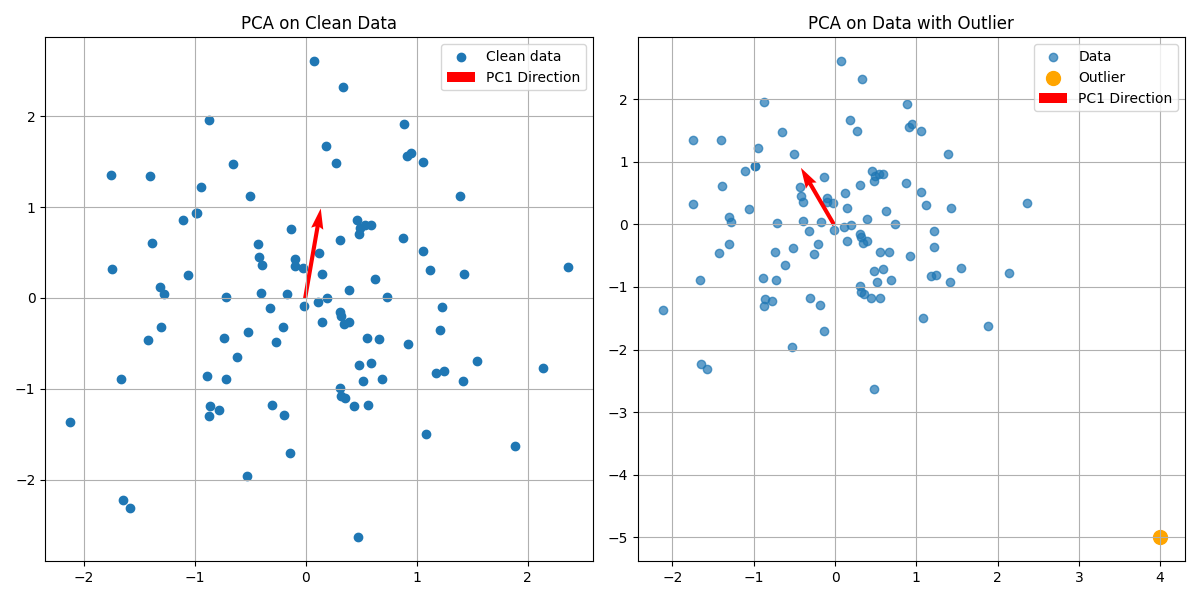
\includegraphics[width=\textwidth]{images/q1-6_pca_plot.png}
    \label{fig:pca_outlier}
\end{figure}

\end{enumerate}


\clearpage

\subsection*{2. Graph Laplacian and GNN [20 points].}
This question is designed to show how Graph Laplacian and the principle of spectral clustering is used in the context of deep learning, in particular, in developing graph neural networks (GNN). In GNN, such as ChebNet (one of the most popular GNNs), filters are defined as \emph{polynomials of the graph Laplacian}, to extract graph features. This question is meant to build the understanding of how properties from Graph Laplacian can be used in GNN. You can refer to the paper referenced below for additional context. \\
Ref: M. Defferrard, X. Bresson, and P. Vandergheynst. Convolutional Neural Networks on Graphs with Fast Localized Spectral Filtering. NeurIPS, 2016.\\

Formally, if $L$ is the graph Laplacian and $T_k(\cdot)$ is the Chebyshev polynomial of order $k$, then
\[
g_\theta(L)\,x \;\approx\; \sum_{k=0}^K \theta_k\, T_k(\tilde{L})\, x,
\qquad \tilde{L}=\tfrac{2}{\lambda_{\max}}L - I .
\]
where $\lambda_{\max}$ is the largest eigenvalue of the Graph Laplacian. 
Here, ``a polynomial applied to the graph Laplacian'' means taking powers of $L$ (e.g., $I, L, L^2,\dots$) and combining them with learnable coefficients $\theta_k$.  
Recall from lecture that $L = D - A$, where $D$ is the degree matrix and $A$ is the adjacency matrix.  

\medskip
\textbf{Example (Chebyshev, small $K$).}  
Take $K=2$ and use $T_0(x)=1$, $T_1(x)=x$, $T_2(x)=2x^2-1$. Then
\[
g_\theta(L)\,x \;\approx\; \theta_0\,T_0(\tilde L)\,x \;+\; \theta_1\,T_1(\tilde L)\,x \;+\; \theta_2\,T_2(\tilde L)\,x.
\]
For a toy 3-node path with
\[
A=\begin{bmatrix}
0&1&0\\
1&0&1\\
0&1&0
\end{bmatrix},\quad
L=D-A=\begin{bmatrix}
1&-1&0\\
-1&2&-1\\
0&-1&1
\end{bmatrix},
\]
one computes
\[
L^2=\begin{bmatrix}
2&-3&1\\
-3&6&-3\\
1&-3&2
\end{bmatrix},\qquad
T_2(L)=2L^2-I=\begin{bmatrix}
3&-6&2\\
-6&11&-6\\
2&-6&3
\end{bmatrix}.
\]
Thus, a single ChebNet layer with $K=2$ applies a learnable combination of $\{x,\;Lx,\;T_2(L)x\}$ to produce updated node features---no eigenvectors required.

\medskip
\textbf{How this is used in a GNN layer.}
\begin{itemize}
    \item \emph{Input:} a matrix $X\in\mathbb{R}^{n\times d}$ of node features (one row per node).  
    \item \emph{Operation:} build $\{T_k(\tilde L)X\}_{k=0}^K$ (each mixes information up to $k$ hops), linearly combine them with learnable weights, and pass througha nonlinearity.  
    \item \emph{Output:} new node features $X'\in\mathbb{R}^{n\times d'}$ that aggregate information from multi-hop neighborhoods.  
\end{itemize}

\medskip
\textbf{Questions.} In this exercise, we will show how GNN is constructed based on the idea of graph Laplacian, the same idea we exploited in spectral cluster. 
\begin{enumerate}[label=(\arabic*)]

    \item (10 Points) \textbf{Neighborhood aggregation.}
    \begin{enumerate}[label=(\alph*)]
        \item Show that 
        \[
        (Lx)_i = d_i x_i - \sum_{j\sim i} x_j,
        \]
        so multiplying by $L$ mixes node $i$’s value with its \textbf{1-hop neighbors}.
        \subsection*{2.a Neighborhood Aggregation Proof}
        To start, we can expand on $Lx$
        \begin{align*}
            Lx &= (D-A)x \\
            &= Dx - Ax
        \end{align*}
        Looking at this logically, $D$ is a degree matrix and $A$ is an adjacency matrix. Multiplying a vector by a diagonal matrix just scales each element $x_i$ by the degree in $D_{ii}$. The same logic can be applied to the adjacency matrix, which contains 1 with 1-hop neighbors, and 0 elsewhere. Therefore, the product with $x$ will sum the values $x_i$ where a 1 is present in the row $A_i$. These operations together are expressed in $d_i x_i - \sum_{j\sim i} x_j$. To show this, we will perform the $Lx$ multiplication and see they are equal.
        \begin{align*}
            Dx = \begin{bmatrix}1&0&0 \\0&2&0 \\0&0&1\end{bmatrix} \begin{bmatrix}x_1\\x_2\\x_3 \end{bmatrix} &= \begin{bmatrix} x_1 \\ 2x_2\\x_3 \end{bmatrix} \\
            -Ax = \begin{bmatrix}0&-1&0 \\-1&0&-1 \\0&-1&0 \end{bmatrix} \begin{bmatrix} x_1\\x_2\\x_3\end{bmatrix} &= \begin{bmatrix} -x_2\\-x_1-x_3\\-x_2 \end{bmatrix} \\
            Lx = \begin{bmatrix} x_1-x_2 \\ -x_1+2x_2-x_3 \\ -x_2+x_3\end{bmatrix}
            \intertext{Now to show $d_ix_i$ and $\sum_{j\sim i} x_j$ are equal to the above:}
            Dx = \begin{bmatrix} x_1 \\ 2x_2 \\ x_3 \end{bmatrix} &= \begin{bmatrix} x_1 \\ 2x_2 \\ x_3 \end{bmatrix} \\
            \sum_{j\sim i} x_j &= \begin{bmatrix} x_2 \\ x_1+x_3 \\ x_2\end{bmatrix} \\
            Dx - \sum_{j\sim i} x_j &= \begin{bmatrix} x_1-x_2 \\ -x_1+2x_2-x_3 \\ -x_2+x_3\end{bmatrix} \\
            \intertext{So we can clearly see:} \\
            (Lx)_i = \begin{bmatrix} x_1-x_2 \\ -x_1+2x_2-x_3 \\ -x_2+x_3\end{bmatrix} = d_i x_i - \sum_{j\sim i} x_j
        \end{align*}
        \item Explain why $L^2 x$ includes terms that traverse \textbf{paths of length up to 2} (so information propagates up to 2-hops). 
        \subsection*{2.b 2 Hop Aggregation}
            \textbf{For reference, here is the graph based on the adjacency matrix}. This image can be used to help visualize the hopping process.
            \begin{figure}[H]
                \centering
                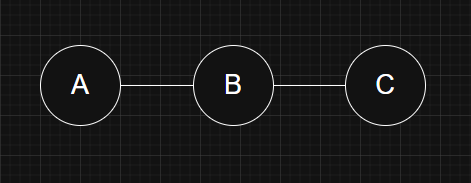
\includegraphics[width=\textwidth]{images/q2_graph.png}
                \label{fig:q2_graph}
            \end{figure}
        We will expand $L^2$ to show that the terms incorporate 2-hop neighbors.
        \begin{align*}
            L^2x &= ((D-A)(D-A))x \\
            ((D-A)(D-A))x &= D^2x - DAx - ADx + A^2x \\
            \intertext{Perform the multiplication on each term using the example matrices:}
            &= \begin{bmatrix}1&0&0\\0&4&0\\0&0&1\end{bmatrix}x- \begin{bmatrix}0&1&0\\2&0&2\\0&1&0\end{bmatrix}x - \begin{bmatrix}0&2&0\\1&0&2\\0&2&0\end{bmatrix}x + \begin{bmatrix}1&0&1\\0&2&0\\1&0&1\end{bmatrix}x
        \end{align*}
        In the above equation, we can see that the $D^2x$ term is scaling by the degree of each node. The $-DAx$ and $-ADx$ terms are dealing with 1-hop neighbors, similar to how we saw in 2.1 with the $Lx$ case. Most interestingly, the $A^2x$ term is the term that incorporates 2-hop neighbors. We can that the following conditions are now non-zero: A connects to C and A, B connects to B, and C connects to C and A. Referencing the graph, we can see that these combinations are all 2-hops. Through these mechanisms, we can see that the $L^2x$ case accounts for path lengths up to 2.
        \item Conclude: why does applying a polynomial in $L$ aggregate information from \textbf{multiple hops} in one shot?
        \subsection*{2.c Polynomial $L$ Aggregation}
        From the expansions of the $L$ equation in 2.a and 2.b, we can see that each power of $L$ incorporates information from an additional hop due to the adjacency matrix terms. Therefore, further power of $L$ will continue incorporating more hops as each power of the adjacency matrix will exist in the expanded polynomial up to the maximum number of hops.
    \end{enumerate}

    \begin{tcolorbox}[colback=gray!10,colframe=gray!60!black,title=Hint]
    Recall: the off-diagonal entries of $L$ are negative when nodes are connected, and diagonal entries contain the degree. 
    Multiplying by $L$ subtracts neighbor contributions and scales by the degree. Multiplying again by $L$ compounds this mixing, reaching farther neighbors.
    \end{tcolorbox}

    \item  (10 Points)  \textbf{Small example calculation.}  
    Using the 3-node path above, compute $L=D-A$. Then, with $T_0(x)=1$, $T_1(x)=x$, $T_2(x)=2x^2-1$, write down $T_2(L)$ explicitly.
    \subsection*{2.2 Validating given calculation}
    \begin{align*}
    L = D-A = \begin{bmatrix}1&0&0 \\0&2&0 \\0&0&1\end{bmatrix} - \begin{bmatrix}1&-1&0 \\-1&2&-1 \\0&-1&1 \end{bmatrix} &= \begin{bmatrix}1&-1&0 \\-1&2&-1 \\0&-1&1 \end{bmatrix} \\
    L^2 &=\begin{bmatrix}2&-3&1\\-3&6&-3\\1&-3&2\end{bmatrix} \\
    T_2(L)=2L^2-I= 2\begin{bmatrix}2&-3&1\\-3&6&-3\\1&-3&2\end{bmatrix}-\begin{bmatrix}1&0&0\\0&1&0\\0&0&1\end{bmatrix} &=\begin{bmatrix}3&-6&2\\-6&11&-6\\2&-6&3\end{bmatrix}
\end{align*}
This matches the given calculation in the problem.
\end{enumerate}

%\clearpage

\subsection*{3. Order of faces using ISOMAP [25 points]}

This question aims to reproduce the ISOMAP algorithm results in the original paper for ISOMAP, J.B. Tenenbaum, V. de Silva, and J.C. Langford, Science 290 (2000) 2319-2323 that we have also seen in the lecture as an exercise (isn't this exciting to go through the process of generating results for a high-impact research paper!) 


The file \textsf{isomap.mat} (or \textsf{isomap.dat}) contains 698 images, corresponding to different poses of the same face. Each image is given as a 64 $\times$ 64 luminosity map, hence represented as a vector in $\mathbb R^{4096}$. This vector is stored as a row in the file. (This is one of the datasets used in the original paper.) In this question, you are expected to implement the ISOMAP algorithm by coding it up yourself. You may find the shortest path (required by one step of the algorithm), using \url{https://docs.scipy.org/doc/scipy/reference/generated/scipy.sparse.csgraph.shortest_path.html}. 


Using Euclidean distance (i.e., in this case, a distance in $\mathbb R^{4096}$) to construct the $\epsilon$-ISOMAP (follow the instructions in the slides.) You will tune the $\epsilon$ parameter to achieve the most reasonable performance. Please note that this is different from $K$-ISOMAP, where each node has exactly $K$ nearest neighbors.

\begin{enumerate} 

\item (5 points) Visualize the nearest neighbor graph through either an image of your adjacency matrix, or visualizing the graph similar to the lecture slides using graph packages such as Gephi (\textsf{https://gephi.org}). Additionally, include a few of the face images that correspond directly to nodes on different parts of your visualization.
 \subsection*{3.1 Nearest Neighbor Graph}

 The first step in creating the nearest neighbor graph is to compute the pairwise distance. Then, we need to find a suitable $\epsilon$ to construct the adjacency matrix. The $\epsilon$ value serves a radius to determine which nodes are close enough to be considered neighbors. If $\epsilon$ is too small, the graph can be entirely disconnected or have suboptimal geodesic distances. If $\epsilon$ is too large, the graph manifold structure can be compromised. To find this, I used the scipy \lstinline{csr_matrix} and \lstinline{connected_components} functions. \lstinline{Connected_components} basically determines how many disconnected graphs are present, so I clearly want $\epsilon$ to be large enough for only 1 component. From there, I was interested in the average degree of the matrix, since I figured geodesic distance approximation would benefit from each node's degree being larger than 1 - with more potential paths from each node, there are more combinations to find the shortest path. Luckily, the smallest $\epsilon$ that connected the graph yielded a large enough average degree, so I chose $\epsilon=11.27$.

 The resultant adjacency matrix is shown below with a heatmap. On the heatmap, purple zones indicate a value of 0, meaning the nodes are not neighbors. The other colors are gradients based on the euclidean distance between the connected nodes. I chose a random set of 10 connected pairs and 10 disconnected pairs and displayed the two images for each pair on the heatmap. The connected pairs are outlined in blue and show clear similarity, proving that the distance metric is working well for neighbors. The disconnected pairs are outlined in red and show clear dissimilarity.

 \begin{figure}[H]
                \centering
                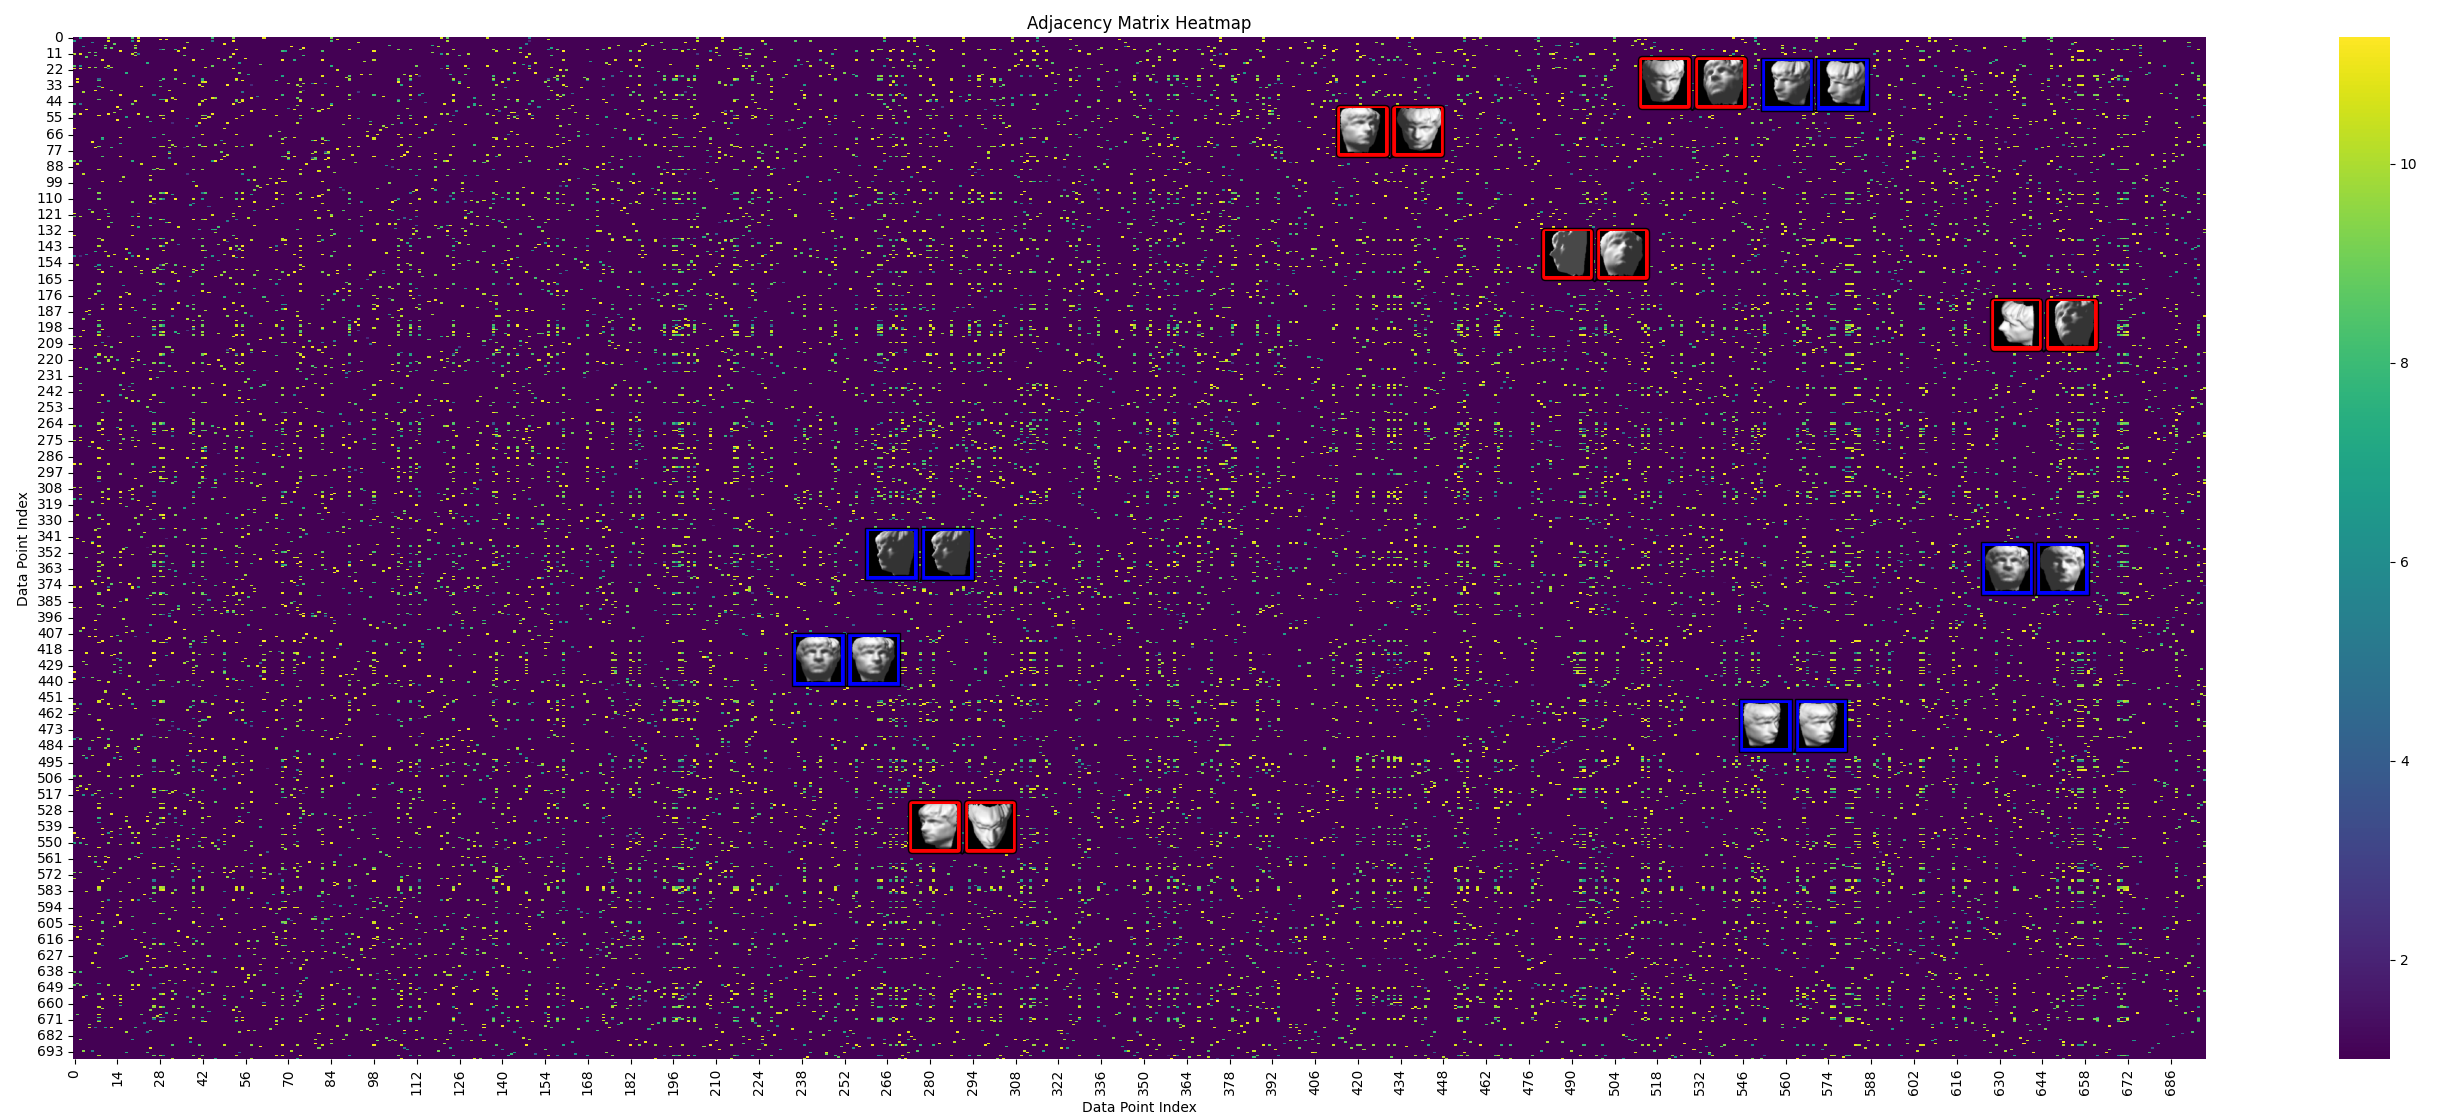
\includegraphics[width=\textwidth]{images/3-1_adjacency_matrix.png}
                \label{fig:q3_adjacency}
            \end{figure}

 \item (10 points) Implement the ISOMAP algorithm yourself to obtain a two-dimensional low-dimensional embedding. Plot the embeddings using a scatter plot, similar to the plots in lecture slides. Find a few images in the embedding space and show what these images look like and specify the face locations on the scatter plot. Comment on do you see any visual similarity among them and their arrangement, similar to what you seen in the paper? Come up with a way to tune the kernel bandwidth to have desired result.
 \subsection*{3.2 ISOMAP 2D Embedding}

 Following the ISOMAP algorithm in the lecture slides, I computed the shortest path distance matrix using the adjacency matrix and the scipy function \lstinline{shortest_path}. Then, I performed the MDS steps in the slides to extract the 2D embedding. The resultant scatter plot is shown below. The displayed faces for 50 random points are shown and have a clear pattern. Not only are similar faces grouped together, but the face orientations are also ordered in a clear circular pattern. Faces facing left are on the left side of the graph and faces facing right are on the right side of the graph. This matches the original ISOMAP results, which is a good sign to see.
 \begin{figure}[H]
                \centering
                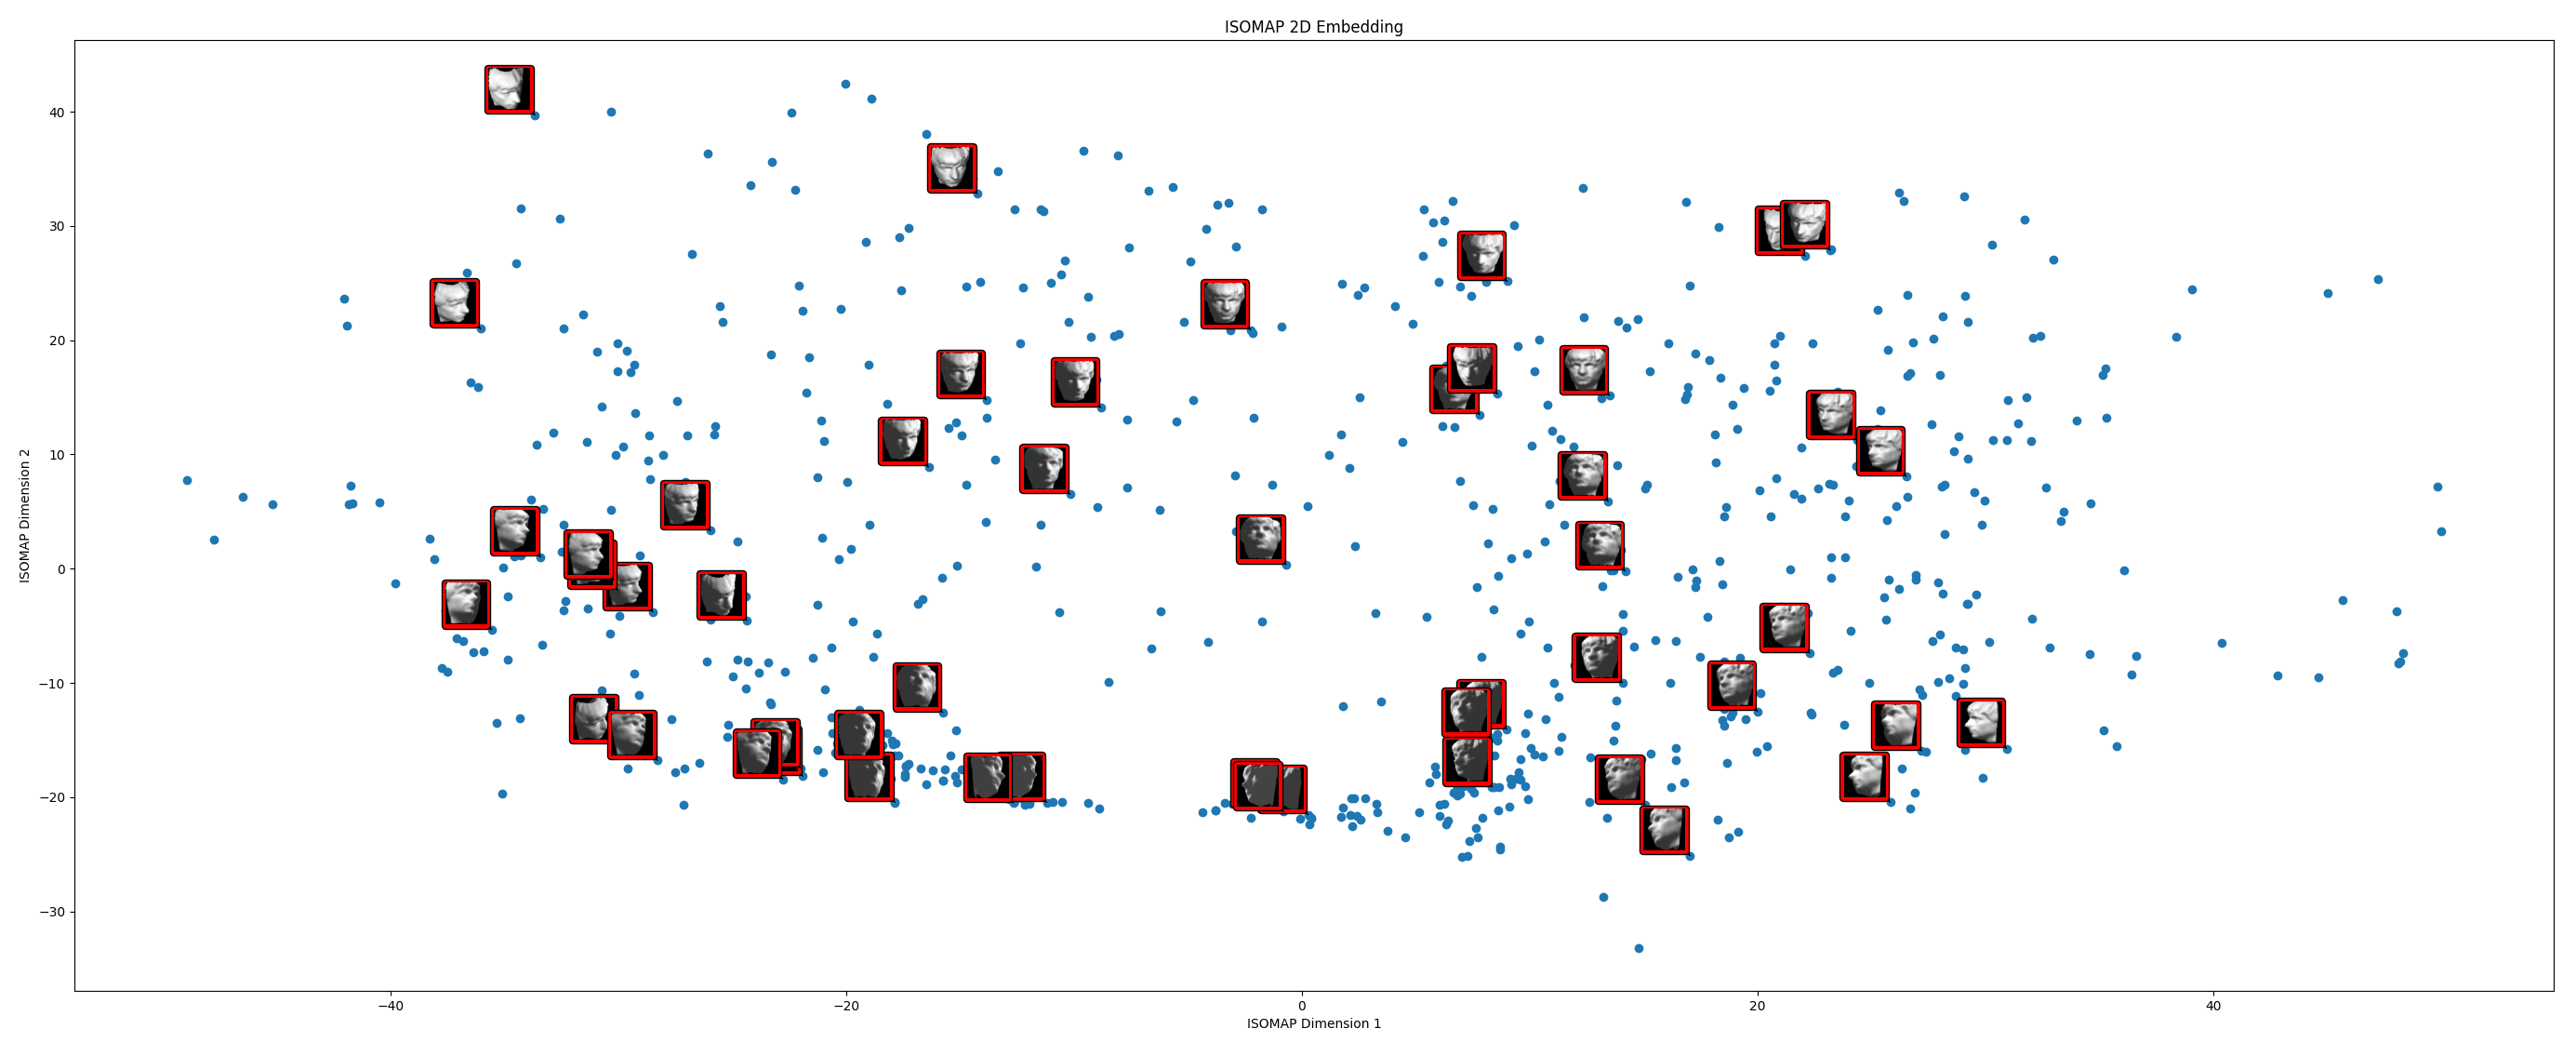
\includegraphics[width=\textwidth]{images/3-2_isomap_embedding.png}
                \label{fig:q3_isomap}
            \end{figure}


\item (10 points) Perform PCA (you can utilize a PCA package for this) on the images and project them into the top 2 principal components. Again show them on a scatter plot. Explain whether or not you see a more meaningful projection using ISOMAP than PCA. 
\subsection*{3.3 PCA 2D Embedding}
To compare dimensionality reduction techniques, I performed PCA using sklearn's \lstinline{StandardScaler} and \lstinline{pca} to reduce the dimensionality to 2D. The resultant scatter plot is shown below. While the faces are generally grouped together, with similar looking faces near each other, the groupings are clearly not as accurate or distinct as the ISOMAP results. Contributing to this, PCA does not produce a good mapping of the orientation of the faces. Visually, a group of example images along Principal Component 1 = -20 show faces oriented in all sorts of directions. This shows that the lienar PCA technique fails to capture the manifold structure of the data (i.e. the circular orientation pattern of the faces).
 \begin{figure}[H]
                \centering
                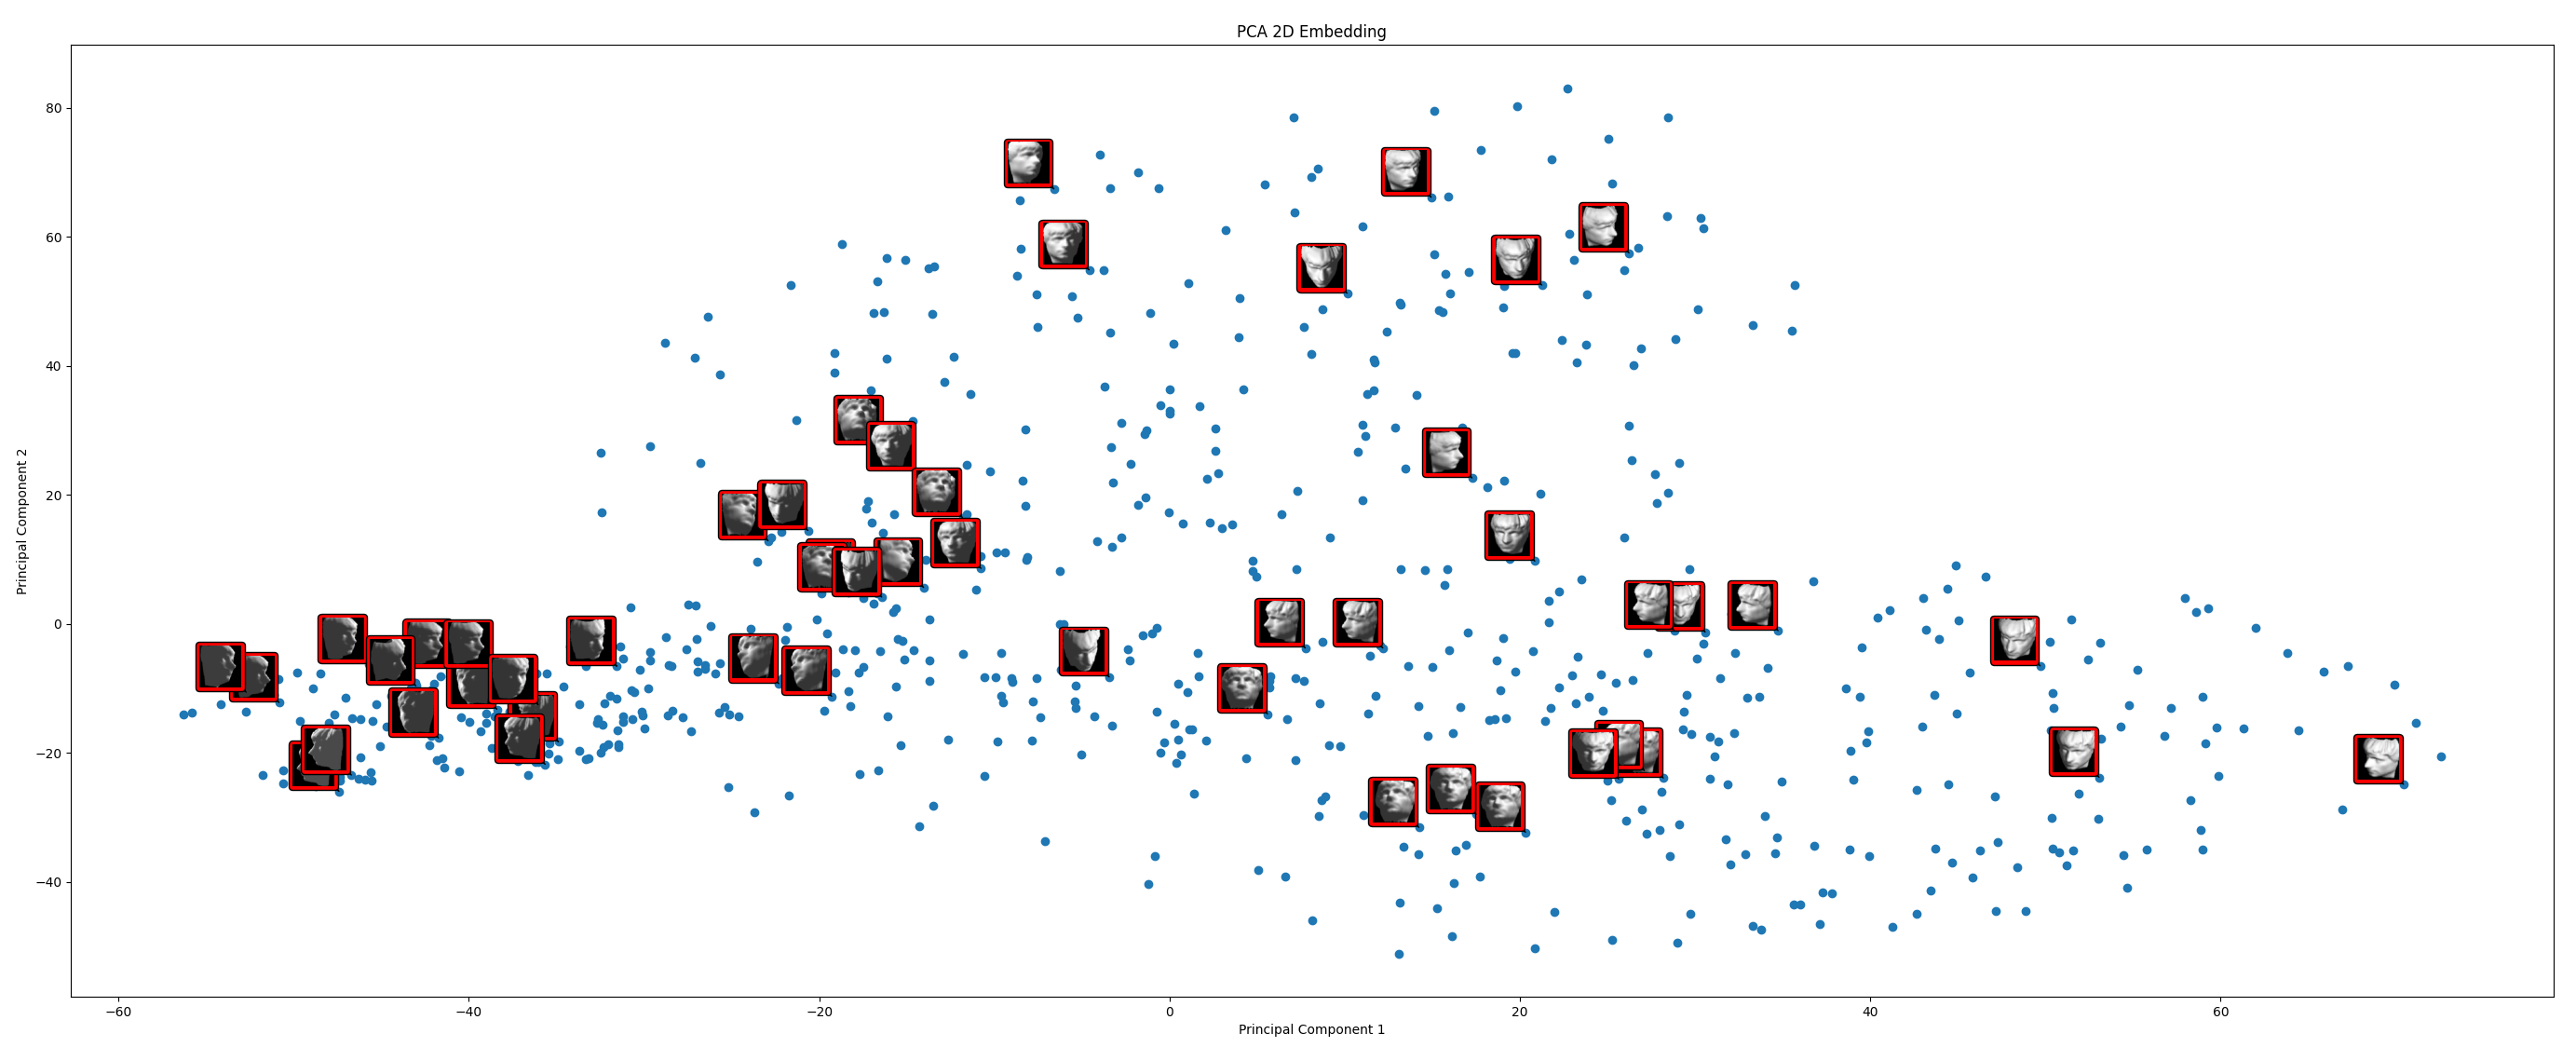
\includegraphics[width=\textwidth]{images/3-3_pca_embedding.png}
                \label{fig:q3_pca}
            \end{figure}
\end{enumerate}




 \clearpage

\subsection*{4. Eigenfaces and simple face recognition [25 points].}

This question is a simplified illustration of using PCA for face recognition. We will use a subset of data from the famous Yale Face dataset. 

\vspace{.1in}
\noindent
{\bf Remark:} You will have to perform downsampling of the image by a factor of 4 to turn them into a lower resolution image as a preprocessing (e.g., reduce a picture of size 16-by-16 to 4-by-4). In this question, you can implement your own code or call packages. 

First, given a set of images for each person, we generate the eigenface using these images. You will treat one picture from the same person as one data point for that person. Note that you will first vectorize each image, which was originally a matrix. Thus, the data matrix (for each person) is a matrix; each row is a vectorized picture. You will find weight vectors to combine the pictures to extract different ``eigenfaces'' that correspond to that person's pictures' first few principal components. 


\begin{enumerate}

\item (10 points) Perform analysis on the Yale face dataset for Subject 1 and Subject 2, respectively, using all the images EXCEPT for the two pictures named \textsf{subject01-test.gif} and \textsf{subject02-test.gif}. {\bf Plot the first 6 eigenfaces for each subject.} When visualizing, please reshape the eigenvectors into proper images. Please explain can you see any patterns in the top 6 eigenfaces?
\subsection*{4.1 Eigenfaces}
To start with this, I procedurally load the images, downsample, and flatten them all in the same way. Then, I use sklearn's \lstinline{StandardScaler} to center the data and Numpy's \lstinline{SVD} to extract the top 6 principal components. I chose SVD because the matrix was wide, which is a better use for SVD versus PCA. I then plotted the top 6 eigenfaces for each subject. Thes results are shown below.
\begin{figure}[H]
                \centering
                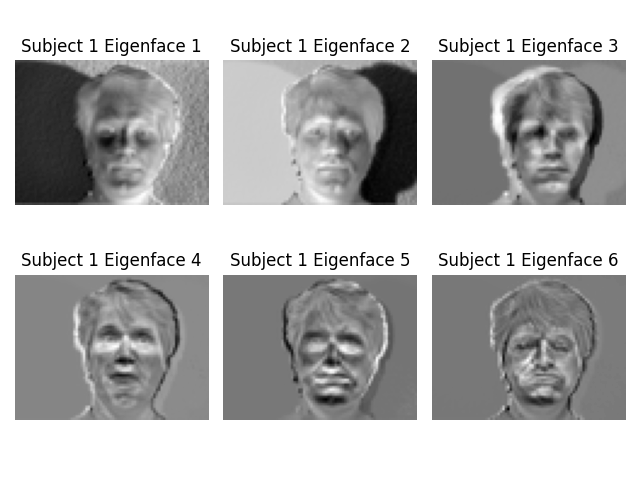
\includegraphics[width=\textwidth]{images/eigenfaces_subject1.png}
                \label{fig:Eigenfaces_Subject1}
            \end{figure}
\begin{figure}[H]
                \centering
                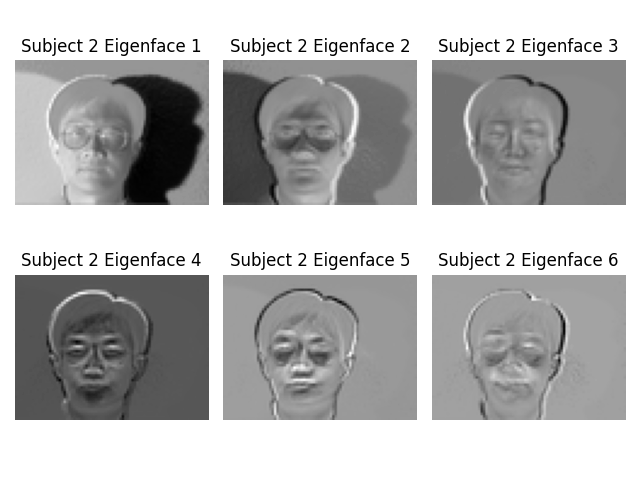
\includegraphics[width=\textwidth]{images/eigenfaces_subject2.png}
                \label{fig:Eigenfaces_Subject2}
            \end{figure}
The eigenfaces seem to get the gist of the subjects' faces. I do notice that the most significant eigenfaces seem to favor any part of the image with hard edges. The gifs with shadows and glasses are very prominent in the top eigenfaces, though there are only 2 training images with shadows and 1 with glasses.

\item (10 points) Now we will perform a simple face recognition task. 

Face recognition through PCA is proceeded as follows. Given the test image \textsf{subject01-test.gif} and \textsf{subject02-test.gif}, first downsize by a factor of 4 (as before), and vectorize each image. Take the top eigenfaces of Subject 1 and Subject 2, respectively. Then we calculate the {\it projection residual} of the 2 vectorized test images with the vectorized eigenfaces:
\[s_{ij} = \|\textsf{(test image)}_j - \textsf{(eigenface}_i)\textsf{(eigenface})_i^T \textsf{(test image)}_j\|_2^2\]

Report all four scores: $s_{ij}$, $i = 1, 2$, $j = 1, 2.$ Explain how to recognize the faces of the test images using these scores. 

\subsection*{4.2 Face Recognition}
The primary concern in this portion is to ensure that the test image is preprocessed in the same way as the training images. This means that the test image should be centered to the mean of the training images, which required me to pass the scaler mean down to this step. The projection residual is then calculated as described and the results are shown below.
 \begin{figure}[H]
                \centering
                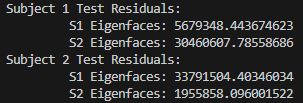
\includegraphics[width=\textwidth]{images/4-2_residuals_results.png}
                \label{fig:q3_pca}
            \end{figure}

From these scores, we can clearly see that the residuals are lowest when the test image and eigenfaces are from the same subject. This makes sense, and we can classify the test image by choosing the subject with the lowest residual.

\item (5 points)
 Comment if your face recognition algorithm works well and discuss how you would like to improve it if possible.

\end{enumerate}

I think the algorithm works well enough - the residuals are clearly different enough to distinguish which test image belongs to which subject. I believe that more training data would be an impactful improvement. Further, I think that the data should be normalized for lighting. Clearly, the shadowed images significantly effect the eigenfaces, so removing that element would help with the pure facial recognition.

\clearpage


\subsection*{5. To subtract or not to subtract, that is the question [Bonus: 5 points].}

In PCA, we have to subtract the mean to form the covariance matrix 
\[
C = \frac 1 m \sum_{i=1}^m (x^i - \mu)(x^i - \mu)^T 
\]
before finding the weight vectors, where $\mu = \frac 1m \sum_{i=1}^m x^i$. For instance, we let
\[
 C w^1= \lambda_1 w^1
\]
where $\lambda_1$ is the largest eigenvalue of $C$, and $w^1$ is the corresponding largest eigenvector.  

Now suppose Prof. X insisting not subtracting the mean, and uses the eigenvectors of 
\[
\tilde C = \frac 1 m \sum_{i=1}^m x^i {x^i}^T
\]
to form the weight vectors. For instance, she lets $\tilde w^1$ to be such that 
\[
\tilde C \tilde w^1 = \tilde \lambda_1 \tilde w^1
\]
where $\tilde \lambda_1$ is the largest eigenvalue of $\tilde C$. 

Now the question is, are they the same (with and without subtract the mean)? Is $w^1$ equal or not equal to $\tilde w^1$? Use mathematical argument to justify your answer.

\subsection*{5.1}
\textbf{I will not be attempting this due to time constraints.}

\printbibliography


\end{document}